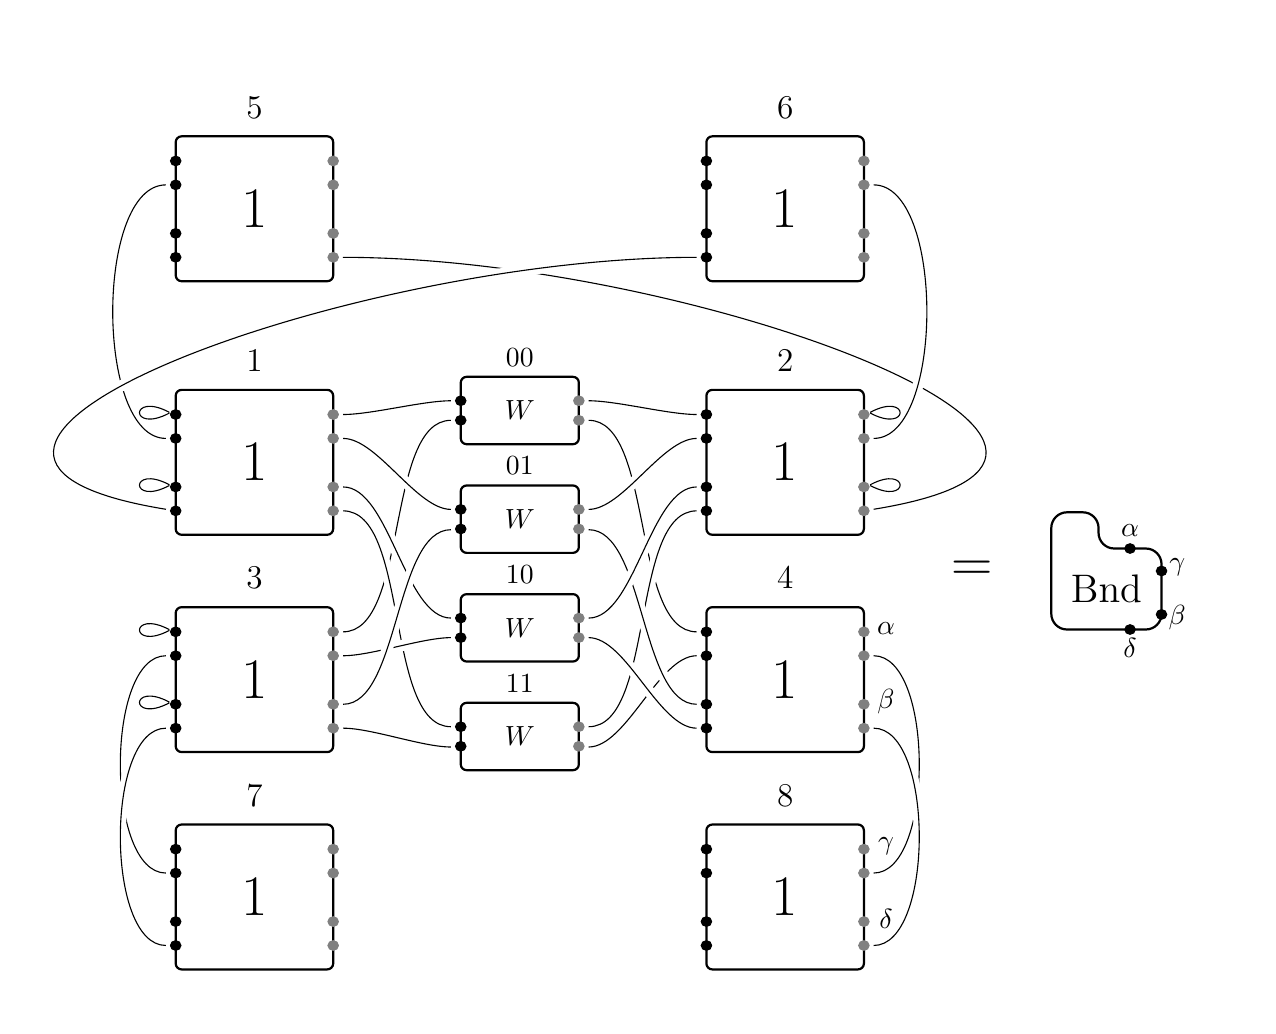
\begin{tikzpicture}[yscale=0.92] 

\path[use as bounding box](-5.5,-3) rectangle (10,10.5);
 % Each Hadamard Rectangle 
\foreach \xshift / \yshift /\xscale / \lab / \unitary in{3.12/0.5/1/4/1,3.12/3.5/1/2/1,-3.62/0.5/1/3/1,-3.62/3.5/1/1/1, -3.62/-2.5/1/7/1,3.12/-2.5/1/8/1, 3.12/7/1/6/1, -3.62/7/1/5/1}
{ 
\begin{scope}[shift={(\xshift,\yshift)},xscale=\xscale]
  \draw[rounded corners=0.75mm,thick] (0,0) rectangle (2 cm, 2cm);
  \node at (1,1) {\huge$\unitary$};   
\node at (1,2.4) {\large\lab};
  \foreach \y in {.33,.66,1.33,1.66}
	{   
		\foreach \x /\color in {0/black,2/gray}
			{    
				\draw[fill=\color,draw=\color] (\x cm, \y cm) circle (.66mm);  
			}
	} 
\end{scope}
}
  % Each W Gadget
\foreach \yshift/\from in {0.25/11,1.75/10,3.25/01,4.75/00}
{ 
\begin{scope}[yshift=\yshift cm] 
 \draw[rounded corners=0.75mm,thick] (0,0) rectangle (1.5cm,.93cm); 
 \node at (.75,.465) {$W$};   
\node at (.75,1.2) {$\from$};
  \foreach \x/\color in {0/black,1.5/gray}
	{   
		\foreach \y in {0.33,.6}
		{   
			 \draw[fill=\color,draw=\color] (\x,\y) circle (.66mm); 
		 }
	}
\end{scope}
}
  % Right Connections
\foreach \l/\r in {   5.35/5.16,5.08/2.16,   .85/3.83,.57/1.83,   3.85/4.83,3.57/1.16,   2.35/4.16,2.08/.83} 
{   
\node (a) at (1.5,\l) {}; 
 \node (b) at (3.12,\r)   {}; 
 \draw[looseness=.66,line width=4pt,color=white] (a) to [out=0,in=180] (b);
  \draw[looseness=.66] (a) to [out=0,in=180] (b); 
}
  % Left Connections
\foreach \l/\r in {5.16/5.35,2.16/5.08,   3.83/.85,.83/.57,   4.83/3.85,1.83/2.08,   4.16/2.35,1.16/3.57}
{   
\node (a) at (-1.618,\l) {}; 
 \node (b) at (0,\r)   {};
  \draw[looseness=.66,line width=4pt,color=white] (a) to [out=0,in=180] (b);
  \draw[looseness=.66] (a) to [out=0,in=180] (b); 
}

%%%%%%%Edges which connect to the two lower diagram elements

%The one on the left-hand side

\node (c) at (-3.62,1.83){};
\node (d) at (-3.62,-1.17){};

 \draw[looseness=.66,line width=4pt,color=white] (c) to [out=180,in=180] (d);
 \draw[looseness=.66] (c) to [out=180,in=180] (d); 

\node (c) at (-3.62,0.83){};
\node (d) at (-3.62,-2.17){};

 \draw[looseness=.66,line width=4pt,color=white] (c) to [out=180,in=180] (d);
 \draw[looseness=.66] (c) to [out=180,in=180] (d); 

% The one on the right-hand side

\node (c) at (5.12,1.83){};
\node (d) at (5.12,-1.17){};

 \draw[looseness=.66,line width=4pt,color=white] (c) to [out=0,in=0] (d);
 \draw[looseness=.66] (c) to [out=0,in=0] (d); 

\node (c) at (5.12,0.83){};
\node (d) at (5.12,-2.17){};

 \draw[looseness=.66,line width=4pt,color=white] (c) to [out=0,in=0] (d);
 \draw[looseness=.66] (c) to [out=0,in=0] (d); 

%%%%%%%Edges which connect to the two upper diagram elements

%The ones on the left-hand side

\node (c) at (-3.62,8.33){};
\node (d) at (-3.62,4.83){};

 \draw[looseness=.66,line width=4pt,color=white] (c) to [out=180,in=180] (d);
 \draw[looseness=.66] (c) to [out=180,in=180] (d); 

\node (c) at (-1.62,7.33){};
\node (d) at (5.12,3.83){};

 \draw[looseness=1.5,line width=4pt,color=white] (c) to [out=0,in=10] (d);
 \draw[looseness=1.5] (c) to [out=0,in=10] (d); 

%The ones on the right-hand side

\node (c) at (5.12,8.33){};
\node (d) at (5.12,4.83){};

 \draw[looseness=.66,line width=4pt,color=white] (c) to [out=0,in=0] (d);
 \draw[looseness=.66] (c) to [out=0,in=0] (d); 

\node (c) at (3.12,7.33){};
\node (d) at (-3.62,3.83){};

 \draw[looseness=1.5,line width=4pt,color=white] (c) to [out=180,in=170] (d);
 \draw[looseness=1.5] (c) to [out=180,in=170] (d); 




  % Node Labels

\draw[looseness=150] (-3.7,5.19) to [out=150,in=210] (-3.7,5.18) ;   
\draw[looseness=150] (-3.7,4.19) to [out=150,in=210] (-3.7,4.18) ;   

\draw[looseness=150] (-3.7,2.19) to [out=150,in=210] (-3.7,2.18) ;   
\draw[looseness=150] (-3.7,1.19) to [out=150,in=210] (-3.7,1.18) ;   

\draw[looseness=150] (5.2,5.19) to [out=30,in=-30] (5.2,5.18) ;   
\draw[looseness=150] (5.2,4.19) to [out=30,in=-30] (5.2,4.18) ;   

\node at (5.4,2.2) {$\alpha$};
\node at (5.4,1.2) {$\beta$};
\node at (5.4,-0.8) {$\gamma$};
\node at (5.4,-1.8) {$\delta$};

  \node at (6.5cm,3cm) {\huge $=$};
\begin{scope}[xshift = 7.5cm,yshift = 3.81cm]       
\draw[rounded corners = 2mm,thick] (0,0) -- (.6,0) -- (.6,-.5) -- (1.4,-.5) -- (1.4,-1.618) -- (0,-1.618) -- cycle;                    \draw[fill=black] (1,-.5) circle (.66mm);             
\draw[fill=black] (1.4,-.81) circle (.66mm);       
\draw[fill=black] (1.4,-1.41) circle (.66mm);       
\draw[fill=black] (1,-1.618) circle (.66mm);              
\node at (1,-.25) {$\alpha$};       
\node at (1.6,-.76) {$\gamma$};       
\node at (1.6,-1.46) {$\beta$};       
\node at (1,-1.868) {$\delta$};              
\node at (.7,-1.06) {\Large Bnd};          
\end{scope}
\end{tikzpicture}